% THIS IS SIGPROC-SP.TEX - VERSION 3.1
% WORKS WITH V3.2SP OF ACM_PROC_ARTICLE-SP.CLS
% APRIL 2009
%
% It is an example file showing how to use the 'acm_proc_article-sp.cls' V3.2SP
% LaTeX2e document class file for Conference Proceedings submissions.
% ----------------------------------------------------------------------------------------------------------------
% This .tex file (and associated .cls V3.2SP) *DOES NOT* produce:
%       1) The Permission Statement
%       2) The Conference (location) Info information
%       3) The Copyright Line with ACM data
%       4) Page numbering
% ---------------------------------------------------------------------------------------------------------------
% It is an example which *does* use the .bib file (from which the .bbl file
% is produced).
% REMEMBER HOWEVER: After having produced the .bbl file,
% and prior to final submission,
% you need to 'insert'  your .bbl file into your source .tex file so as to provide
% ONE 'self-contained' source file.
%
% Questions regarding SIGS should be sent to
% Adrienne Griscti ---> griscti@acm.org
%
% Questions/suggestions regarding the guidelines, .tex and .cls files, etc. to
% Gerald Murray ---> murray@hq.acm.org
%
% For tracking purposes - this is V3.1SP - APRIL 2009

\documentclass{acm_proc_article-sp}
%\usepackage[dvips]{graphicx}
%\usepackage[fleqn]{amsmath}
%\usepackage{amsthm}
%\usepackage{txfonts}
\usepackage{courier}
\usepackage{subfigure}
\usepackage{comment}
\usepackage{url}
\usepackage[square,numbers]{natbib}

%-----------------------------------------
% need for camera-ready
\pagestyle{empty}

%----------------------------------------

\begin{document}

\title{
Towards Adaptive GPU Resource Management for Embedded Real-Time Systems
}
%
% You need the command \numberofauthors to handle the 'placement
% and alignment' of the authors beneath the title.
%
% For aesthetic reasons, we recommend 'three authors at a time'
% i.e. three 'name/affiliation blocks' be placed beneath the title.
%
% NOTE: You are NOT restricted in how many 'rows' of
% "name/affiliations" may appear. We just ask that you restrict
% the number of 'columns' to three.
%
% Because of the available 'opening page real-estate'
% we ask you to refrain from putting more than six authors
% (two rows with three columns) beneath the article title.
% More than six makes the first-page appear very cluttered indeed.
%
% Use the \alignauthor commands to handle the names
% and affiliations for an 'aesthetic maximum' of six authors.
% Add names, affiliations, addresses for
% the seventh etc. author(s) as the argument for the
% \additionalauthors command.
% These 'additional authors' will be output/set for you
% without further effort on your part as the last section in
% the body of your article BEFORE References or any Appendices.

\numberofauthors{2} %  in this sample file, there are a *total*
% of EIGHT authors. SIX appear on the 'first-page' (for formatting
% reasons) and the remaining two appear in the \additionalauthors section.
%
\author{
% You can go ahead and credit any number of authors here,
% e.g. one 'row of three' or two rows (consisting of one row of three
% and a second row of one, two or three).
%
% The command \alignauthor (no curly braces needed) should
% precede each author name, affiliation/snail-mail address and
% e-mail address. Additionally, tag each line of
% affiliation/address with \affaddr, and tag the
% e-mail address with \email.
%
\alignauthor Junsung Kim\\
       \affaddr{Dept. of Electrical and Computer Engineering}\\
       \affaddr{Carnegie Mellon University}\\
       \email{junsungk@cmu.edu}
\alignauthor Ragunathan (Raj) Rajkumar\\
       \affaddr{Dept. of Electrical and Computer Engineering}\\
       \affaddr{Carnegie Mellon University}\\
       \email{raj@ece.cmu.edu}
\and
\alignauthor Shinpei Kato\\
       \affaddr{Dept. of Information Engineering}\\
       \affaddr{Nagoya University}\\
       \email{shinpei@is.nagoya-u.ac.jp}
}
% There's nothing stopping you putting the seventh, eighth, etc.
% author on the opening page (as the 'third row') but we ask,
% for aesthetic reasons that you place these 'additional authors'
% in the \additional authors block, viz.
%\additionalauthors{Additional authors: John Smith (The Th{\o}rv{\"a}ld Group,
%email: {\texttt{jsmith@affiliation.org}}) and Julius P.~Kumquat
%(The Kumquat Consortium, email: {\texttt{jpkumquat@consortium.net}}).}
%\date{30 July 1999}
% Just remember to make sure that the TOTAL number of authors
% is the number that will appear on the first page PLUS the
% number that will appear in the \additionalauthors section.

\maketitle

%-----------------------------------------
% need for camera-ready
\thispagestyle{empty}

\begin{abstract}
 In this paper, we present two conceptual frameworks for GPU applications to
 adjust their task execution times based on total workload. These  
 frameworks enable smart GPU resource management when many applications 
 share GPU resources while the workloads of those applications vary. 
 Application 
 developers can explicitly adjust the number of GPU cores depending on their needs. 
 An implicit adjustment will be supported by a run-time framework, which 
 dynamically allocates the number of cores to tasks based on the total 
 workload. The runtime support of the proposed system can be realized using 
 functions which measure the execution times of the tasks on GPU and change 
 the number of GPU cores. We motivate the necessity of this framework 
 in the context of self-driving technologies, and we believe that our 
 frameworks for GPU programming are useful contributions given 
 the increasing emphasis on 
 %trends are apparently shifting to highly 
 parallel heterogeneous computing.
\end{abstract}

\section{Introduction}
\label{sec:introduction}

Graphics processing units (GPUs) are becoming more and more commonplace
in many application domains widely ranging from high-performance
computing to embedded mobile computing.
For example, three of the top five supercomputers on the TOP500
list~\cite{TOP500}, announced as of March 2012, use GPUs to accelerate
computations, while recent tablets, such as ASUS Eee Pad Transformer
Prime, also leverage embedded GPUs, like Tegra
3~\cite{Tegra3}, to enhance performance under power constraints.
This trend is expected to continue. 

One notable application domain of GPUs is automotive engineering.
Modern automobiles employ several tens of processing units.
Further advances in safe-driving features, such as adaptive
cruise control, stop-and-go cruise control, lane keeping, and assisted
lane change, would require even larger computing capabilities.
%As vehicles are becoming autonomous, 
For vehicles to become fully or semi-autonomous, 
a multitude of computer vision,
sensor fusion, signal processing, and graphics sub-systems must operate and
communicate in real-time~\cite{Kelly12, Markoff10, Urmson08}.
Given their highly data-parallel and compute-intensive workloads, 
parallel computing is a useful solution.
As technology stands today, the GPU is the most well-suited platform.
In fact, NVIDIA GPUs will be used for infotainment systems platforms in
future product lines of BMW vehicles~\cite{NVIDIA_BMW}.

%Recent trends in autonomous-driving vehicles~\cite{Kelly12, Markoff10,
%Urmson08} are motivated by various benefits of automated functions,
%but, most importantly, enabling 
Automatic safety features require smart planning and intelligent
processing of data obtained from many sensors equipped in the vehicle,
including LIDAR (LIght Detection And Ranging), radar, camera, and
ultrasonic sensors. 
One common characteristic in these types of processing is that GPUs can
accelerate their processing speeds significantly.
For example, autonomous driving should ideally follow the best path among
many potential paths, whose calculations can happen in parallel.
Calculating as many potential paths to follow as possible
will yield better quality of driving.
As a matter of fact, CMU's autonomous vehicle team showed that their
motion planning algorithm was sped up by 40 times~\cite{McNaughton11},
using an NVIDIA GTX 260 GPU that integrates 192 compute cores on a
chip.

In addition to motion planning, a perception algorithm as well as 
sensor data processing can benefit from the GPU.
The perception system of a self-driving car should
be able to detect, classify and track the obstacles around
itself. Various types of sensors will generate voluminous amount of
information that must be processed in order to understand the vehicle's surroundings. 
%In order to process the data, a parallel processing technique is of vital importance. 
For example, a self-driving car at CMU manages 1536 objects from LIDAR
sensors before they are fused with other types of sensor data. There has
been on-going research using GPU to build a perception
system~\cite{Ferreira11}, and their GPU implementation yielded
30,000-times-faster performance compared to the case of using only one CPU. 

As described above, there has been research on applying GPU to different applications on self-driving cars, and it is clear that GPU can provide great benefits on realizing safer or self-driving car technologies. However, not much research has been done when those technologies are deployed together on self-driving cars, where the loads of each application dynamically vary depending on the environment. The period and the computation time of the planning algorithms for autonomous driving highly depend on the vehicle speed, so the planning algorithms can be heavily loaded when the car is (say) on a highway. The load of the perception algorithms mainly depends on the number of obstacles around the car. Hence, the perception system requires more computing resources when the car is driving in an urban area. Therefore, an intelligent method of sharing many cores on GPU would be essential when we use GPUs on self-driving cars. For example, if a self-driving car has a 96-core GPU, the planning algorithm of the car can use 72 cores on the highway and use 12 cores in the urban environment. A self-driving car~\cite{Urmson08} requires tens of tasks, and the dynamic core management should be fulfilled across all tasks if those tasks utilize GPU. 

In this paper, we present two conceptual frameworks for
GPU applications to adjust their task execution times 
given current workload conditions. These frameworks enable
smart GPU resource management when many applications
share GPU resources while the workloads of those applications vary. 
These frameworks support both explicit and implicit adjustment. 
With support for explicit adjustment, %we provide API functions so that 
application developers can adjust the number
of GPU cores depending on their needs. %An implicit adjustment will provide 
A run-time framework will dynamically
allocate the number of cores to tasks based on current 
workloads. The runtime support of our proposed system
can be realized using functions which measure the execution 
times of the tasks on GPU and change the number of cores.

The rest of paper is organized as
follows. Section~\ref{sec:system_model} describes how our proposed
system is modeled. Section~\ref{sec:adaptivity_support} presents the
methods for managing GPU resources in an adaptive manner, and we conclude our paper in Section~\ref{sec:summary}.

\section{System Model}
\label{sec:system_model}

We assume real-time embedded systems that contain CPU and one or more GPUs as compute devices.
An application task starts execution on the CPU, and offloads its
data-parallel compute-intensive workload onto the GPU when needed.
Once offloaded onto the GPU, the task becomes non-preemptive due to many
reasons.
In fact, it is technically possible to preempt the running task on the
GPU by loading and restoring its context, but it requires additional
firmware, runtime, and OS support, and the preemption cost would be
non-trivial due to a very large set of GPU registers and states.
We, hence, restrict our attention to a non-preemptive execution model for
GPU computing.
GPUs may also pose some constraints in multi-tasking.
Even the NVIDIA Fermi architecture~\cite{Fermi}, one of the most popular
GPU product lines, allows only one context to use GPU resources at
once, though this context may spawn multiple GPU kernels (jobs)
simultaneously.
In other words, if task-level parallelism is required, the entire system
must run in the same context.
We, however, believe that this constraint will not limit the 
concepts we describe in this paper.
The same GPU context can be used to exploit concurrent parallel job
executions, to serve at least as a proof of concept. 
We also expect that future product lines will remove this concern.

We consider real-time applications where each task runs in a periodic or
sporadic manner under deadline constraints.
Such a task set may include motion planning and 
vision-based perception in state-of-the-art autonomous driving
vehicles, where the periods often correspond to frame-rates, and the
deadlines occur at the end of the period.
%It should however be noted that deadline constraints may not be relevant
%to periods depending on applications, but the computation must meet the
%deadline in order to achieve the desired quality of service in either case.
We also presume that the computing demand of each task is highly
variable.
For example, the performance of planning and perception tasks is usually
governed by the number of objects, the size of data, and the desired
quality of output.
These workloads are also very parallelizable using the GPU.
%Hence, the autonomous driving tasks and applications are our primary
%target, but 
The contributions of this paper are not limited to autonomous driving tasks but
are also generally applicable to highly variable workloads running on the
GPU.

\section{Adaptive GPU Resource Management}
\label{sec:adaptivity_support}

In this section, we describe adaptive support for GPU applications.
We particularly focus on solving resource allocation problems.
The goal is to support embedded real-time systems that exhibit highly variable
workloads.
Since GPUs integrate a large number of cores on a chip, 
we aim to enable the execution of 
highly variable workloads in a timely manner by adjusting
allocated cores at runtime.

Several approaches have been studied for adaptive GPU resource
management.
Some work~\cite{Kato_RTAS11, Kato_RTSS11, Kato_ATC11} took
time-driven approach that controls timings and the duration of time
allowed to access GPU resources, \textit{i.e.}, scheduling and
reservation.
In these time-driven approaches, application tasks need not to be aware
of what is happening in GPU resource management, because it is handled
by the OS or runtime scheduler.
However, they can not manage task execution times.
They also limit the number of contexts that can access the GPU
simultaneously to remove performance interference.
Therefore, GPU resources could be wasted if a running context does not
fully use compute cores.

We consider a different approach than previous work that enables GPU
applications to adjust their task execution times.
The number of cores used in the program is a major
factor that affects the execution time. Hence, we explore how to
adjust the core allocation at runtime.
It is important to note that the programmer is typically responsible for
allocating the number of cores (or threads mapped to cores) in GPU
programming.
In order to adjust the number of cores at runtime, it is essential to
provide the programmer with an interface to obtain the information on
the number of cores available or allocated for the program at runtime.
The programmer is then responsible for making the program adaptive to
the number of cores.

\begin{figure}[t]
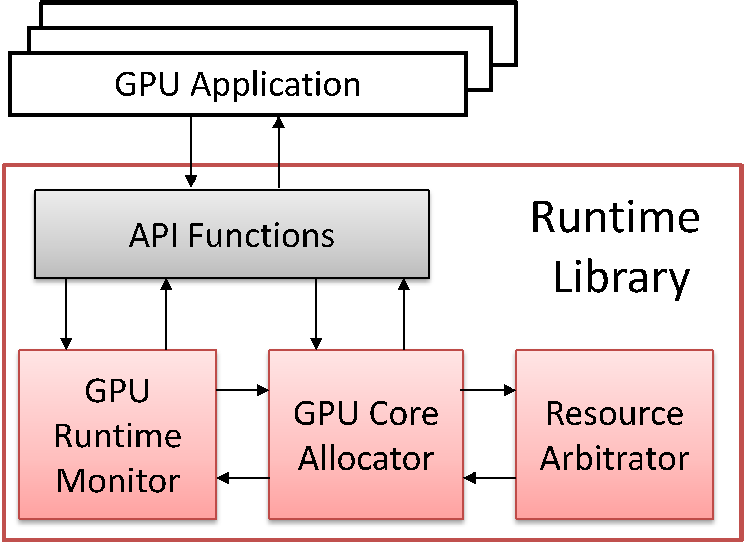
\includegraphics[width=3.0in]{architecture.eps}
\caption{The proposed conceptual architecture for GPU resource management.} 
\label{fig_arch}
\end{figure}

In the following, we present two frameworks that could be used to 
implement the proposed approach. 
%Although they are still at an idea stage, 
We plan to implement a real
system as a proof-of-concept, leveraging open-source
software~\cite{Kato_OSPERT11}. The proposed architecture is also 
illustrated in Figure~\ref{fig_arch}.

\subsection{Explicit Adjustment}

In our explicit adjustment framework, the programmer is
responsible for adjusting the number of cores to relax or tighten
the computing demand.
There will be no adjustment unless the programmer explicitly takes an
action.
A typical usage of this framework with periodic real-time tasks is as
follows.

At the end of each period, the programmer calls a function provided
by our framework that returns the latest task execution time.
The programmer next calls either of the following two API functions.
One increases the number of cores to be used by the next GPU execution 
to speed up the program.
The other decreases it to slow down the program.
This framework is usable in practice because the programmer often knows the
desired task execution time to meet the frame-rate or deadline.
It is also flexible in that the programmer can determine when to
increase or decrease the number of cores.

A downside of this framework is that a task may misbehave
and interfere with other contending application tasks, if the programmer
fails to call the API functions correctly.
We can cap the maximum number of cores available for an individual task
to prevent it from abusing GPU resources, but the adaptive nature of computing
depends on the programmer, and outside system control.

\subsection{Implicit Adjustment}

Our second approach to adaptive resource management is an implicit
adjustment framework.
In this framework, the number of cores to be allocated for the program
is set by the runtime system.
Hence, the adaptivity of computing does not really depend on the programmer.
If the program is not aware of this framework, however, it may fail to
run, since the number of core allocated for the program may be different
from what the program assumes.

The programmer specifies the desired task execution time as a set point
before the task starts.
If this set point is not specified, the runtime system tries to derive
it internally as time goes by.
When the task uses the GPU, the runtime system consistently updates the
number of cores available for the corresponding task in the next period
based on the previous execution time records.
It is still the programmer's duty to check the number of available cores before
offloading the computation onto the GPU.

This implicit adjustment framework is more preferable to the explicit
adjustment framework, as it can enforce adaptive GPU resource
management.
However, it requires consensus in the programming model that the number
of cores allocated for the program could be changed every time it is
offloaded onto the GPU, and the programmer must be aware of it to make
the program work.
We claim that this is a natural trade-off between the generality of
programming and needed adaptivity of service.

\subsection{Runtime System Support}
\label{sec:runtime}

The runtime system provides the API for real-time GPU programmers.
In order to support adaptive GPU resource management, we must provide
some additional API functions.

\begin{itemize}
 \item Our adaptive GPU resource management frameworks require a
       function to measure the execution time of each job running on the
       GPU.
       This function is easy to implement.
       Since we assume that job execution on the GPU is non-preemptive,
       the amount of time in run-to-completion can be accounted as job
       execution time.
       This accounting method is also known to work from previous
       studies~\cite{Kato_ATC11, Rossbach_SOSP11}.
       For the explicit adjustment framework, this function must be
       exposed to the programmer, while it is used internally
       by the implicit adjustment framework.
 \item We also need several functions to change the number of cores to
       be allocated for the program.
       Some existing programming languages for GPGPU, \textit{e.g.},
       CUDA~\cite{CUDA}, provide the API to allow the programmer to
       specify the shape of the grid structure and the number of threads
       mapped to compute cores.
       We can use this API as it is, or provide a corresponding API if
       the underlying programming language does not support it.
\end{itemize}

In addition to these API functions, the runtime system must be able to
detect when the program is offloaded onto the GPU and when it is
completed on the GPU.
Since the programmer calls a specific API function to launch the GPU
program in most GPU programming models, it is very easy to record the
start time of GPU execution.
The detection of the completion time of GPU execution, on the other hand, is
not straightforward.
We would need to use an interrupt to notify the runtime system of
the completion of GPU execution.
Polling on a particular register is an alternative, but it
would not be suitable for latency-sensitive real-time systems, as
previous work demonstrated~\cite{Kato_ATC11}.

Finally, runtime system support must be integrated with the API so that
the programmer can make use of our frameworks under a single unified
programming model.
We plan to extend our CUDA runtime library developed in previous
work~\cite{Kato_OSPERT11} to support our adaptive frameworks.
While this is our planned prototype implementation, and our frameworks can also be
integrated with other programming models beyond CUDA.

\section{Summary}
\label{sec:summary}

In this paper, we have discussed adaptivity requirements in embedded
real-time systems with GPUs, and presented two frameworks for adaptive
GPU resource management.
We conjecture that the generality of programming may need to be compromised
to achieve adaptivity of resource allocation on the GPU.
Nonetheless, adaptive resource management is a key solution in
optimizing performance under resource-constrained environments.
We believe that our frameworks for GPU programming are useful
contributions in this line of work, given the increasing emphasis in 
highly parallel heterogeneous computing.

In future work, we plan to integrate our frameworks into our prototype
fault-tolerant adaptive systems~\cite{Kim_RTSS12} for autonomous driving
technology.
This is highly a challenging project to coordinate high-performance and
adaptive computing for embedded real-time applications.

\bibliographystyle{plain}
{\footnotesize
\bibliography{references}
}

\end{document}
